\documentclass[11pt]{beamer}
\title{Incorrectness Logic}
\usepackage{verbatim}
\usepackage{amsmath}
\usepackage{amsthm}
\usepackage{graphics}
\usepackage{color}
\usepackage{stmaryrd}

\newtheorem{proposition}{Proposition}


\author{Peter W. O'Hearn}
\date{\today}


\begin{document}
\maketitle
\begin{frame}\frametitle{Overview}
\begin{itemize}
\item Intuitive Introduction to Incorrectness Logic
\item Incorrectness Logic: Syntax and Proof Rules
\item Incorrectness Logic: Semantic 
\item Reasoning with the Logic
\end{itemize}
\end{frame}
\begin{frame}\frametitle{Incorrectness Logic: Intuitive Introduction}

This paper describes a simple logic for program incorrectness which is the other side of the coin to Hoare's logic of correctness.

Hoare's Logic:
\begin{center}
$\{precond\}code\{postcond\}$
\end{center}
where $postcond$ is an \textbf{over-approximation(superset)} of the final states reachable.

Incorrectness Logic: 
\begin{center}
$[presumption]code[result]$

\end{center}
where $result$ is a \textbf{under-approximation(subset)} of the final states reachable. 
\end{frame}

\begin{frame}\frametitle{Why Incorrectness Logic?}
As is known, Hoare's logic is used to prove that programs do not contain bugs.

Incorrectness logic, however, is used  to prove the presence of bugs but not their absence. 

\begin{center}
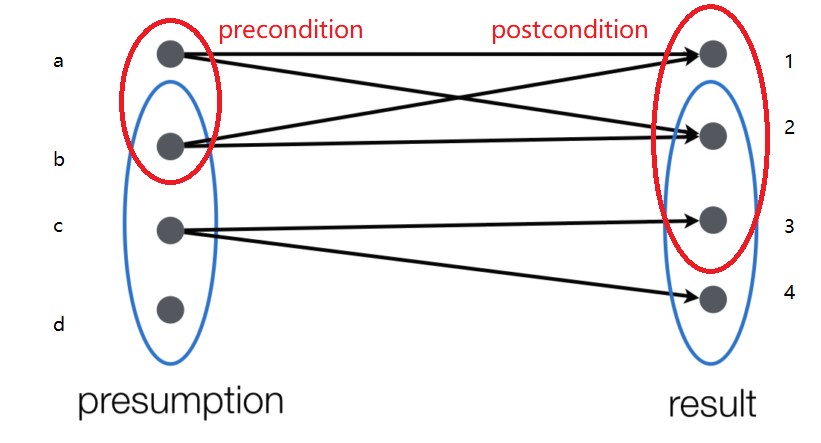
\includegraphics[scale = 0.30]{1.PNG}

\end{center}
\end{frame}
\begin{frame}
\begin{center}
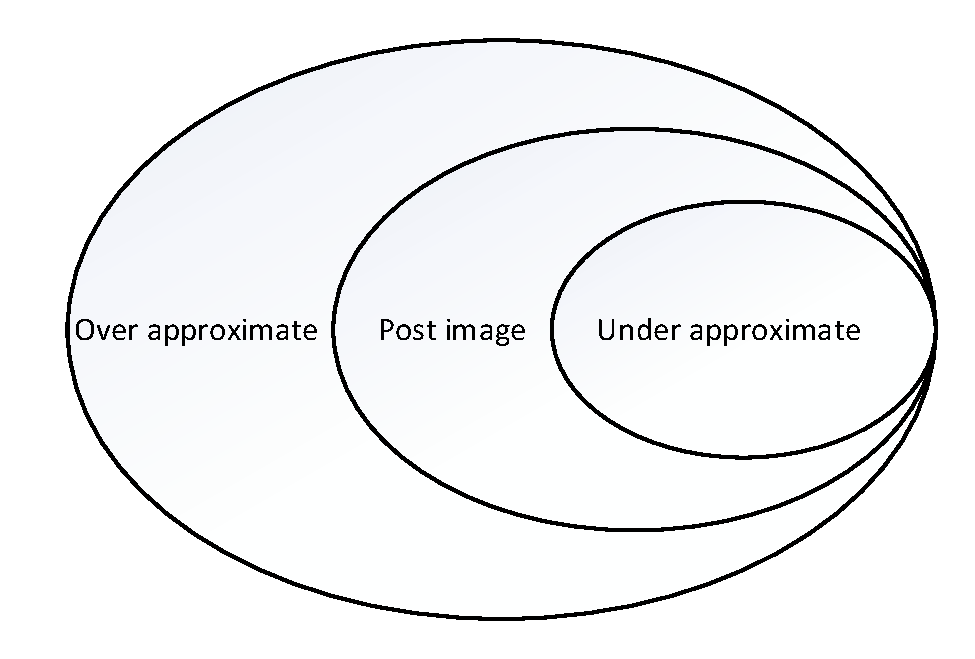
\includegraphics[scale = 0.6]{1.pdf}

\end{center}

\end{frame}
\begin{frame}\frametitle{Toolset}

Website: \underline{fbinfer.com}
\begin{center}
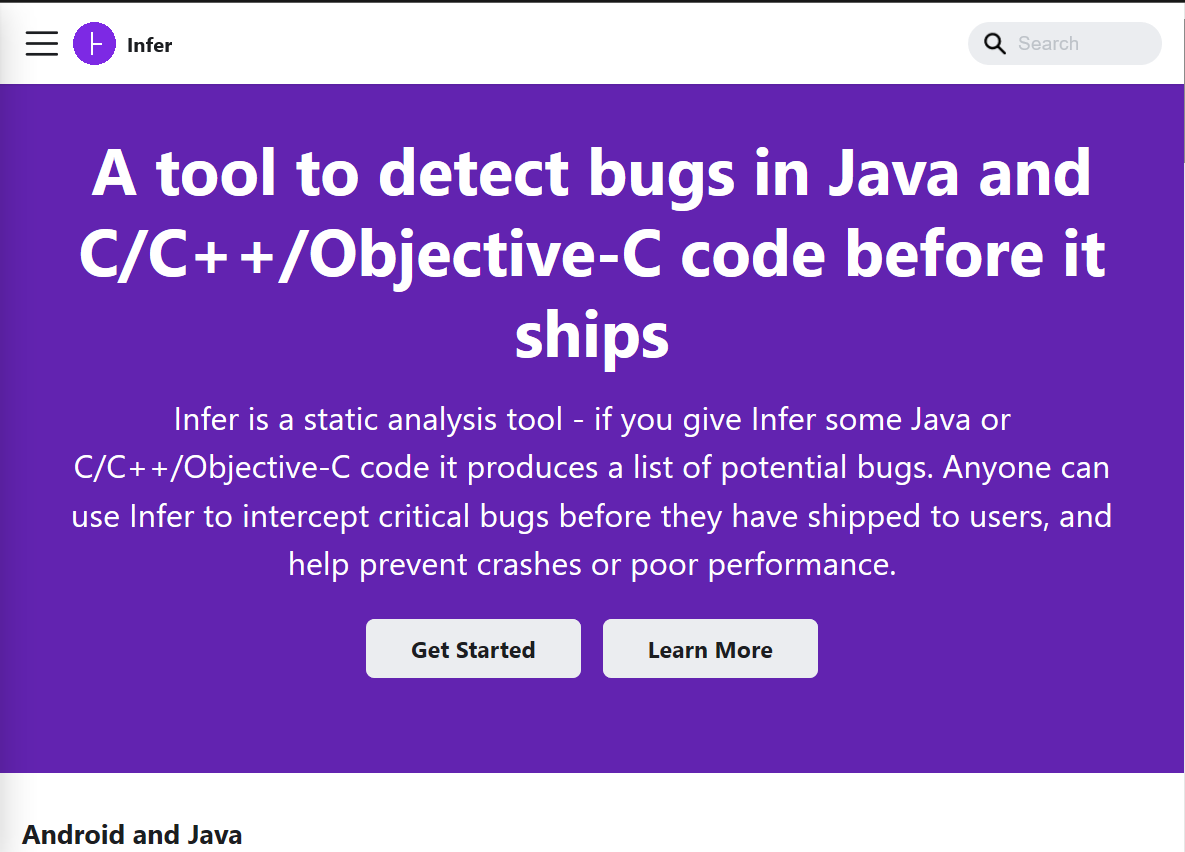
\includegraphics[scale=0.35]{infer.png}

\end{center}

\end{frame}

\begin{frame}\frametitle{Examples}
\textbf{Under-approximating Triples}

For incorrectness logic, we use ``presume" as to identify a pre-assertion and use ``achieves" to identify the post-assertion. Consider an example below.
\begin{center}
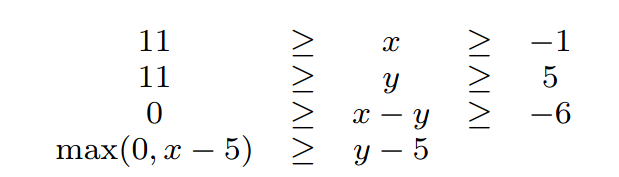
\includegraphics[scale = 0.25]{4.png}

\end{center}
Question: is the assertion $z==42$ an under-approximation of the states reachable from executing code from states statisfying the presumption?
\begin{center}
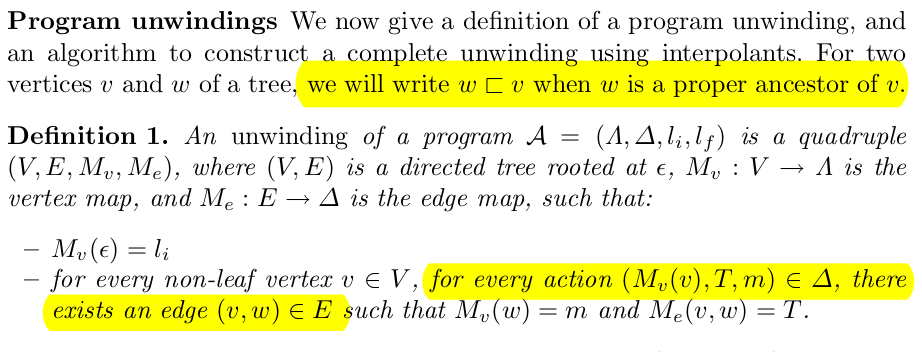
\includegraphics[scale = 0.35]{3.png}
\end{center}
\end{frame}

\begin{frame}\frametitle{Intuition: Inference}
Inference rule of Hoare's logic:
\[\dfrac{\{p\}C\{q\wedge r\}}{\{p\}C\{q\}}\]
where the post condition $q\wedge r$ can be relieved to $q$.

Inference rule of Incorrectness logic:
\[\dfrac{[p]C[q_1 \vee q_2]}{[p]C [q_1]}\]
where the result can only be strengthened. 
\end{frame}

\begin{frame}\frametitle{Examples}
\textbf{Specifying Incorrectness}

We can reason about errors by distinguishing the result-assertion by some tags.
For example, we use ``er: predicate" for erroneous or abnormal termination.
\begin{center}

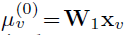
\includegraphics[scale = 0.35]{5.png}

\end{center} 
In this paper, the author only considers errors caused by statement \texttt{error();}.
\end{frame}

\begin{frame}\frametitle{Examples}
\textbf{Under-approximate Success}

Similar to the incorrectness specification, we also need tags for normal, not exceptional, termination of a program. Here we use ``ok" for this purpose.
\begin{center}

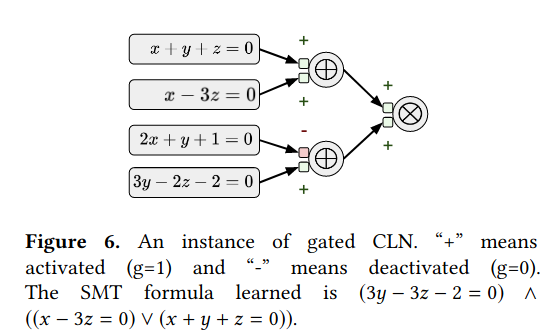
\includegraphics[scale = 0.35]{6.png}

\end{center} 
\end{frame}

\begin{frame}\frametitle{Incorrectness Logic: Syntax and Proof Rules}
Let $\epsilon$ range over a collection of exit conditions, to include at lease ``ok" and ``er". An \textit{under-approximate triple} is of the form:
\[[p]C[\epsilon: q]\]
meaning q under-approximates the states when $C$ exits via $\epsilon$ starting form states in $p$.

Sometimes, we write $[p]C\color{teal}{[ok:q]}\color{red}{[er:r]}$ as shorthand for $[p]C\color{teal}{[ok:q]}$ and $[p]C\color{red}{[er:r]}$


An important point: the triple $[p]C[\epsilon: q]$ express the reachability property that involves termination. \textbf{Every state in the result is reachable from some states in the presumption}
\end{frame}

\begin{frame}\frametitle{Proof Rules}
\begin{itemize}
\item \textit{Empty under-approximate}: $[p]C[\epsilon: false]$

\item \textit{Unit}:
\[[p]skip\color{teal}{[ok:p]}\color{red}{[er:false]}\]

\item \textit{Consequence}:
$\dfrac{p'\Leftarrow p, [p]C[\epsilon: q], q\Leftarrow q'}{[p']C[\epsilon: q']}$

\item \textit{Disjunction}

\[\dfrac{[p_1]C[\epsilon:q_1], [p_2]C[\epsilon: q_2]}{[p_1 \vee p_2]C[\epsilon: q_1 \vee q_2]}\]

\item \textit{Sequencing(short-circuit)}

\[\dfrac{[p]C_1\color{red}{[er:r}]}{[p]C_1;C_2\color{red}{[er:r}]}\]

\item \textit{Sequencing(normal)}

\[\dfrac{[p]C_1\color{teal}{[ok:q}]\color{black}, [q]C_2[\epsilon: r]}{[p]C_1;C_2[\epsilon:r]}\]
\end{itemize}
\end{frame}

\begin{frame}\frametitle{Proof Rules}
\begin{itemize}
\item \textit{Iterate zero}:
$[p]C^\star\color{teal}{[ok:p}]$

\item \textit{Iterate non-zero}:
$\dfrac{[p]C^\star;C[\epsilon:q]}{[p]C^\star;[\epsilon:q]}$
\item \textit{Backwards Variant}:
\[\dfrac{[p(n)\wedge nat(n)]C\color{teal}{[ok:p(n+1)\wedge nat(n)}]}{[p(0)]C^\star\color{teal}{[ok:\exists n.p(n)\wedge nat(n)}]}\]
\item \textit{Choice($i=1$ or $2$)}:
$\dfrac{[p]C_i[\epsilon:q]}{[p]C_1 + C_2[\epsilon:q]}$

\item \textit{Error}: $[p]\texttt{error()}\color{teal}{[ok:false]}\color{red}{[er:p]}$

\item \textit{Assume}: $[p]\texttt{assume } B[\color{teal}{ok:p\wedge B}]\color{red}{[er:false]}$


\end{itemize}
\end{frame}

\begin{frame}\frametitle{Program Conversion}
\begin{center}
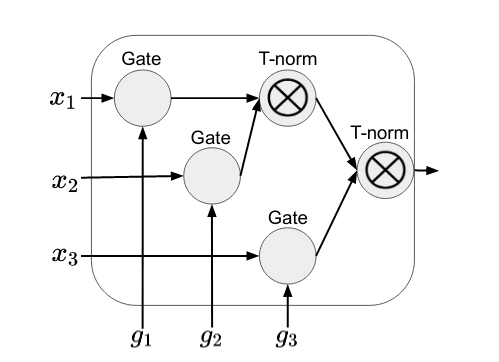
\includegraphics[scale = 0.30]{7.png}

\end{center}

\end{frame}
\begin{frame}\frametitle{Rules for Variables and Mutations}
\begin{center}
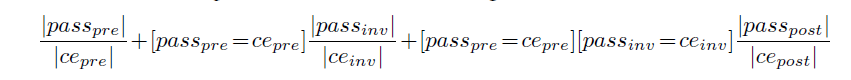
\includegraphics[scale = 0.30]{8.png}

\end{center}
where $Mod(C)$ is the set of variables that program $C$ modified, $Free(r)$ means the set of free variables in assertion $r$ and \texttt{nondet()} is a nondeterministic value.
\end{frame}
\begin{frame}\frametitle{Incorrectness Logic: Semantics}
A set of \textit{states} $\Sigma$ is a set of function from the set \textit{Variables} to the set \textit{Value}.(When reason about termination \textit{Value} is the set of natural numbers).

\begin{definition}[Post and Semantic Triples]
For any relation $r\subseteq \Sigma \times \Sigma$ and predicate $p,q\subseteq \Sigma$ define
\begin{itemize}

\item the \textit{post-image} of $r$, $post(r)\in P(\Sigma)\rightarrow P(\Sigma)$:
\[post(r)p = \{\sigma'\mid \exists \sigma \in p. (\sigma, \sigma')\in r\}\]
\item the \textit{under-approximate triple}:

$[p]r[q]$ is true iff $q\subseteq post(r)p$

\item the \textit{over-approximate triple}(Hoare's logic):

$\{p\}r\{q\}$ is true iff $post(r)p \subseteq q$
\end{itemize}


\end{definition}



\end{frame}

\begin{frame}\frametitle{}

\begin{lemma}[Characterization]
The following statements are equivalent:
\begin{itemize}
\item $[p]r[q]$ is true.
\item $\forall \sigma_q \in q. \exists \sigma_p\in p. (\sigma_p,\sigma_q)\in r$.

\end{itemize}

\end{lemma}

The semantic of the triple $[p]C[\epsilon: q]$? Relations can be regarded as the semantic of a program. Here $\epsilon\in \{ok,er\}$, hence $\llbracket C\rrbracket ok$ and $\llbracket C \rrbracket er$ are two different relations related to program $C$.




\end{frame}

\begin{frame}
\begin{center}\frametitle{Semantics}
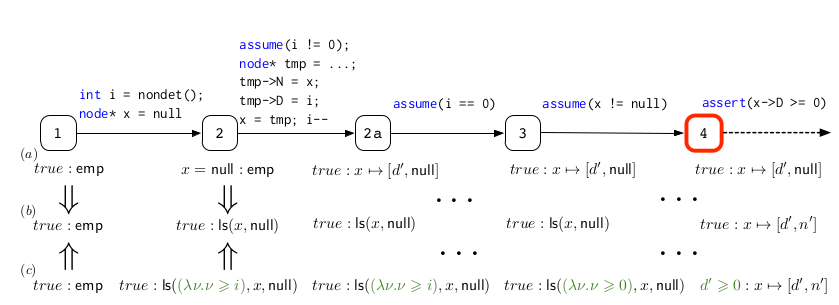
\includegraphics[scale = 0.3]{9.png}
\begin{theorem}
All the listed properties in last section are true of the semantic.

\end{theorem}
\end{center}
\end{frame}

\begin{frame}\frametitle{Soundness and Completeness}
\begin{definition}[Interpretation of Specifications]
$[p]C[\epsilon: q]$ is true iff the semantic triple $[p](\llbracket C\rrbracket \epsilon)[q]$ holds.

\end{definition}


\begin{theorem}[Soundness]
The relational semantics last page validates all the rules introduced before: each axiom is true and each inference rule preserves truth.

\end{theorem}
\begin{theorem}[Completeness]
Every true triple involving finitely-supported predicates is provable.

\end{theorem}
where \textit{finitely-supported} predicate means the predicate only related to finite number of variables in set $Variables$.
\end{frame}

\begin{frame}\frametitle{Predicate Transformers}
Predicate transformers are fundamental semantic tool in  program logic and analysis, which are defined as functions that map predicates to predicates.
\begin{itemize}

\item Forward Transformers. As is known $post(r)p$ can be given as the strongest predicate satisfying $\{p\}r\{q\}$. Symmetricly, we also have the weakest under-approximation to characterize that.
\begin{definition}
For $r\subseteq \Sigma \times \Sigma$:

$StrongestOverPost(r)p = \bigwedge \{q\mid \{p\}r\{q\} holds\}$


$WeakestUnderPost(r)p = \bigvee \{q\mid [p]r[q] holds\}$

\end{definition} 

\begin{proposition}
$StrongestOverPost(r)p = WeakestUnderPost(r)p = post(r)$

\end{proposition}
\end{itemize}

\end{frame}

\begin{frame}\frametitle{Forward Transformer}
Iteration:
\[StrongestOverPost(\llbracket C^*\rrbracket ok)p = \bigwedge \{ I\mid p\Rightarrow I\wedge \{I\}C\{I\} \text{is true}\}\]

\[WeakestUnderPost(\llbracket C^*\rrbracket ok)p = \bigvee_{i\in Nat} \{q\mid [p]C^i[\epsilon:q] \text{is true}\}\]


\[\underline{UnderPost}(\llbracket C^*\rrbracket \epsilon)p = \bigvee_{i\le bound} \{q\mid [p]C^i[\epsilon:q] \text{is true}\}\]

Nondeterministic choice: 

\[post(\llbracket C_1 + C_2 \rrbracket \epsilon) p = post(\llbracket C_1 \rrbracket \epsilon) p \vee post(\llbracket C_1 \rrbracket \epsilon) p\]


\[\underline{post}(\llbracket C_1 + C_2 \rrbracket \epsilon) p = \underline{post}(\llbracket C_1 \rrbracket \epsilon) p \underline{\vee} \underline{post}(\llbracket C_1 \rrbracket \epsilon) p\]


where $p\underline{\vee}q \Rightarrow p\vee q$

\end{frame}

\begin{frame}\frametitle{Backward Transformers}
\begin{fact}[Valid presumptions need not exist]
Given a relation $r$ and assertion $q$, there needs not exist any $p$ such that $[p]r[q]$ holds.

\end{fact}
Strongest under-approximate presumptions do not exists in general.

\begin{example}
$C = (\texttt{assume  x == 1; x = 88}) + (\texttt{assume  x == 2; x = 88})$

\end{example}
\end{frame}

\begin{frame}\frametitle{Reasoning with the Logic}

\[[p]foo()\color{teal}[ok:q]\color{red}[er:s]\color{black} \vdash [p']C\color{teal}[ok:q']\color{red}[er:s']\]






\end{frame}
\begin{frame}\frametitle{Reasoning Details}
\textbf{Reasoning about Loops}

\begin{center}
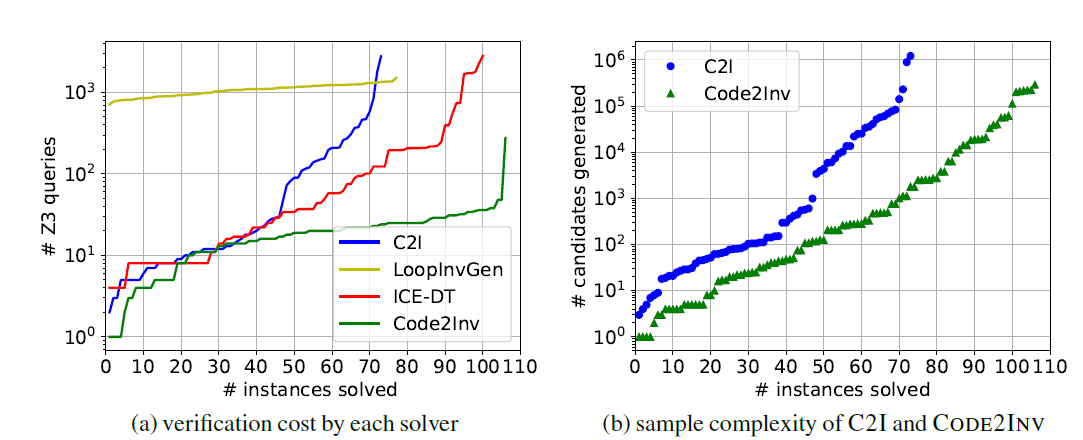
\includegraphics[scale = 0.28]{10.png}

\end{center}
Use consequence rule and implication backward:
\[\dfrac{[true]\texttt{loop0()}\color{teal}{[ok:x \ge 0]}, \color{black}x \ge 0 \Leftarrow x \texttt{==} 2000000}{[true]\texttt{loop0()}\color{teal}{[ok: x \texttt{==} 2000000]}}\]
\end{frame}

\begin{frame}\frametitle{Unroll Loop}

\begin{center}

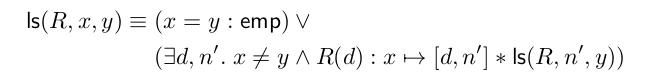
\includegraphics[scale=0.4]{11.png}
\end{center}
\begin{center}

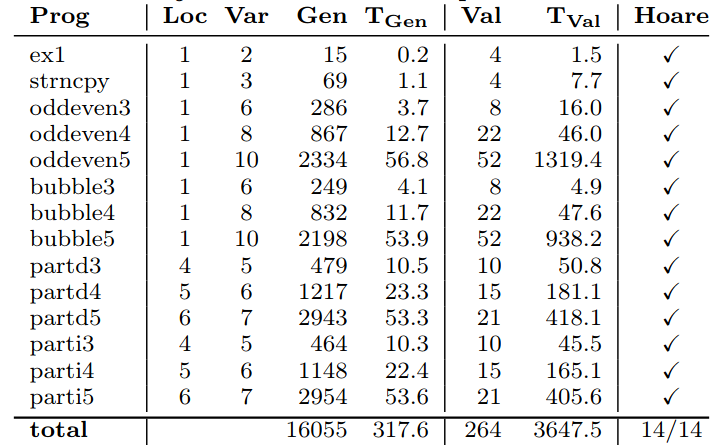
\includegraphics[scale=0.25]{12.png}
\end{center}


\end{frame}

\begin{frame}
\textbf{Conditionals, Expressiveness and Pruning}
\begin{center}

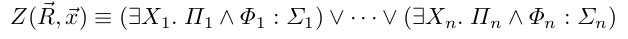
\includegraphics[scale = 0.34]{13.png}
\end{center}
\end{frame}

%\begin{frame}
%\textbf{Symbolic Reasoning and Flaky Tests}

%A "flaky test" is one that, due to nondeterminism, can give different answers on different test runs. "Sturdy" however means that the program give the same answer on all runs of a program.
%\begin{center}

%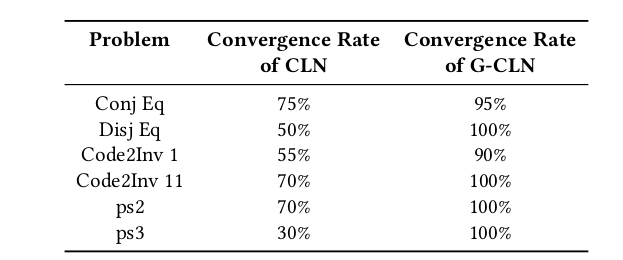
\includegraphics[scale = 0.36]{14.png}
%\end{center}
%\begin{itemize}
%\item $wp(\pi)q$ describe states for which execution of $\pi$ is guaranteed to terminate and satisfy $q$.
%\item $wpp(\pi)q$ describe states for which execution of $\pi$ is possible to terminate and satisfy $q$.

%\end{itemize}
%\end{frame}


\begin{frame}\frametitle{Conclusion}
This paper,
\begin{itemize}
\item described how  under-approximate triples are relevant to proving the presence of bugs,
\item designed a specific logic along with a semantics and proof theory,
\item explored reasoning techniques that are concerned with automatic program analysis.

\end{itemize}

\end{frame}
\end{document}